\documentclass[compress]{beamer}
\usepackage{graphicx}
\usepackage{color}
\usepackage{verbatim}
\usepackage{amsmath}
\usepackage{bm}

%\usetheme{Frankfurt}
%\usecolortheme{lily}

%\useoutertheme[subsection=true]{smoothbars}
\useoutertheme[subsection=true]{miniframes}
\usecolortheme{whale}
\usecolortheme{orchid}
\useinnertheme{rounded}


\newcommand{\xx}{\textbf{r}}

\title{A Classical Density-Functional Theory for Describing Water
  Interfaces}

\author{Jessica Hughes, Eric Krebs, David Roundy}

\date{February 27, 2012}

\setbeamertemplate{navigation symbols}{}

\begin{document}

\begin{frame}
  \titlepage
\end{frame}

\begin{frame}{Outline}
  \tableofcontents
\end{frame}

\section{Methods}

\subsection{Statistical Associating Fluid Theory}

\begin{frame}{}
  SAFT models fluids that have strong association interactions
  (i.e. hydrogen bonding).

  \begin{block}{The SAFT Helmholtz free energy}
    \begin{equation*}
      A = A_\text{id} + A_\text{hs} + A_\text{assoc} + A_\text{disp}
    \end{equation*}
  \end{block}

  \vfill

  We use the optimized SAFT-VR model for water from Clark \emph{et
    al.}$^1$ in the homogeneous limit.  This reproduces water's
  equation of state moderately well away from the critical point.

  \vfill

  \scriptsize{$^1$G.N.I. Clark, A.J. Haslam, A. Galindo, and 
    G. Jackson.\\ \emph{Molecular Physics}, 104(22):3561-3581, 2006.}
\end{frame}

%% \begin{frame}[fragile]{}
%% \begin{figure}
%% \begin{center}
%% \includegraphics[width=\columnwidth]{figs/temperature-versus-density}
%% \end{center}
%% \end{figure}
%% \end{frame}


\begin{frame}[fragile]{}
\begin{figure}
\begin{center}
\includegraphics[width=\columnwidth]{figs/pressure-with-isotherms-truncated}
\end{center}
\end{figure} 
\end{frame}

\newcommand\rr{\mathbf{r}}

\subsection{Classical density-functional theory}

\begin{frame}{Classical density-functional theory}

  \begin{block}{}
    Once we construct a classical density functional, we can find the
    free energy and equilibrium density of a fluid from its external
    potential:
    \begin{equation*}
      A(T) = \underset{n(\xx)}{min}\left\{ F[n(\xx),T] + \int V_{ext}(\xx) n(\xx)
      d^3r\right\}
    \end{equation*}
  \end{block}
  This allows us to address arbitrary \emph{inhomogeneous} density
  distributions.  The challenge is to construct a good functional.

  \vfill

  We have constructed a functional the reproduces the bulk properties
  of the optimized SAFT-VR model of Clark \emph{et al}.

\end{frame}

\begin{frame}[fragile]{}
  \begin{block}{Free energy functional}
    \begin{equation*}
      F[n] = F_\text{id}[n] + F_\text{hs}[n] + F_\text{assoc}[n]  + F_\text{disp}[n]
    \end{equation*}
  \end{block}
  \begin{itemize}
  \item $F_\text{id}[n]$: Ideal gas free energy (the only \emph{local}
    term)
  \item $F_\text{hs}[n]$: Hard sphere excess free energy\\

    We use the White Bear fundamental-measure theory functional, which
    is using convolved densities such as
    \begin{align*}
      n_3(\rr) &= \int n(\rr') \Theta(|\rr-\rr'|-R) d\rr'
    \end{align*}
    $n_2(\rr)$, $n_1(\rr)$, etc. are defined similarly.
  \item $F_\text{assoc}[n]$: Association contribution adapted from Yu
    and Wu$^1$
  \item $F_\text{disp}[n]$: Dispersion contribution (see next slide)
  \end{itemize}

  \vfill

  \scriptsize{$^1$Y.X. Yu and J. Wu., J. Chem. Phys., \textbf{116},
    7094 (2002).}
\end{frame}
 
%% \begin{frame}[fragile]{Association Free Energy}
%%   The association term models the hydrogen bonds as four association
%%   sites on the surface of the hard sphere.  We use the association
%%   functional of Yu and Wu$^1$, modified to use a SAFT-VR model.

%%   \vfill

%%   \scriptsize{$^1$Y.X. Yu and J. Wu., J. Chem. Phys., \textbf{116},
%%     7094 (2002).}

%%   %% \begin{block}{}
%%   %%   \vspace{-1em}
%%   %%   \begin{align*}
%%   %%     F_\text{assoc}[n] &= 4 k_BT \int n_0(\xx)\zeta(\xx)
%%   %%     \left(\ln X(\xx) - \frac{X(\xx)}{2} + \frac12\right) d\xx \\
%%   %%     X(\xx) &= \frac{\sqrt{1 + 8n_0(\xx)\zeta(\xx)
%%   %%         \Delta(\xx)} - 1}
%%   %%     {4 n_0(\xx)\zeta(\xx)
%%   %%       \Delta(\xx)} \\
%%   %%     \Delta(\xx) &= \kappa g^{\text{SW}}_\sigma(\xx)\left(e^{-\beta\epsilon} - 1\right)
%%   %%   \end{align*}
%%   %% \end{block}
%%   %% Here $g^{\text{SW}}_\sigma$ is the correlation function evaluated at contact

%%   %% The functional $X$ is the fraction of association sites \emph{not}
%%   %% hydrogen-bonded.  We use the functional of Yu and Wu$^1$ for the
%%   %% correlation function at contact
%% \end{frame}

\begin{frame}[fragile]{Dispersion Free Energy}
  The dispersion free energy includes any orientation-independent
  interactions. We use a dispersion term based on the SAFT-VR
  approach, with the filling fraction $\eta$ replaced by a convolved
  density
  \begin{align*}
    \eta(\rr) &= \frac{4\pi R^3}{3} \int n(\rr')
    \frac{e^{-\frac{|\rr-\rr'|^2}{2\sigma^2}}}{8\pi^\frac32\sigma^3} d\rr'
  \end{align*}
  where $\sigma$ is an additional empirical parameter used to fit the
  bulk surface tension.
\end{frame}

\begin{frame}[fragile]{}
\begin{figure}
\begin{center}
\includegraphics[width=\columnwidth]{figs/surface-tension}
\end{center}
\end{figure} 
\end{frame}



\section{Results}
%% \subsection{Single hydrophobic rod}

%% \begin{frame}{}
%% \begin{columns}
%%  \column {0.5\textwidth}
%%   \begin{figure}
%%   \begin{center}
%%   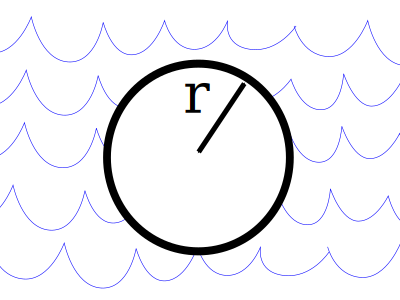
\includegraphics[width=4.5cm]{../papers/thesis-hughes/figs/single-rod-diagram}
%%   \end{center}
%%   \end{figure}
%%   Cross section diagram of a single hydrophobic rod in water.
%%  \column {0.5\textwidth}
%%   \begin{itemize}
%%   \item Pressure = 1~atm
%%   \item Temperature = 298~K
%%   \item Lattice spacing $\approx$~0.01~nm 
%%   \item Radius = 0~nm to 1.5~nm
%%   \end{itemize}
%% \end{columns}
%% \end{frame}

%% \begin{frame}[fragile]{}
%% \begin{figure}
%% \begin{center}
%% \includegraphics[width=\columnwidth]{figs/density-single-rod}
%% \end{center}
%% \end{figure}
%% \end{frame}

%% \begin{frame}[fragile]{}
%% \begin{figure}
%% \begin{center}
%% \includegraphics[width=\columnwidth]{figs/energy-vs-diameter}
%% \end{center}
%% \end{figure} 
%% \end{frame}


\subsection{Two hydrophobic rods}

\begin{frame}[fragile]{}
Two hard purely hydrophobic rods in water.
\begin{figure}
\begin{center}
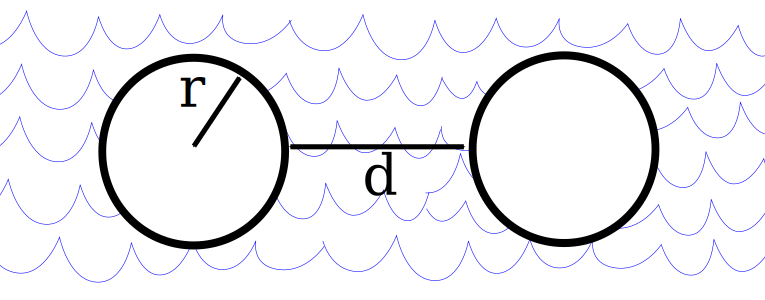
\includegraphics[width=\columnwidth]{figs/rods-diagram}
\end{center}
\end{figure}
We vary the radius $r$ from 0.1~nm to 1.0~nm and the separation $d$
from 0~nm to about 1.2~nm.
\end{frame}

\begin{frame}[fragile]{1 nm  rod diameter}
\begin{columns}
 \column{0.7\textwidth}
  \begin{figure}
  \includegraphics[width=7.3cm]{figs/density-rods-in-water}
  \end{figure} 
 \column{0.3\textwidth}
 \small{``Stadium''-shaped vapor-filled area between rods}\\
 \vspace{0.3cm}
 \small{$d=$~0.5~nm}\\
 \vspace{1.4cm}
 \small{Liquid-filled area between two rods}\\
 \vspace{0.3cm}
 \small{$d=$~0.6~nm}
\end{columns}
\end{frame}

\begin{frame}[fragile]{}
  \begin{columns}
    \begin{column}{0.5\columnwidth}
      \begin{block}{A simple surface-tension model}
        \begin{itemize}
        \item Free energy of the rods $\approx$ surface area times surface tension
        \item Surface tension of bulk water = 72 mN/m
        \item Circumference of the stadium shape:
          \begin{equation*}
            C_{s} = 2\pi r +4r+2d
          \end{equation*}
        \item Circumference of two circles:
          \begin{equation*}
            C_{c} = 4\pi r
          \end{equation*}
        \end{itemize}
      \end{block}
    \end{column}
    \begin{column}{0.5\columnwidth}
      \includegraphics[width=\columnwidth]{figs/rods-energy-vs-distance}

      \vfill

      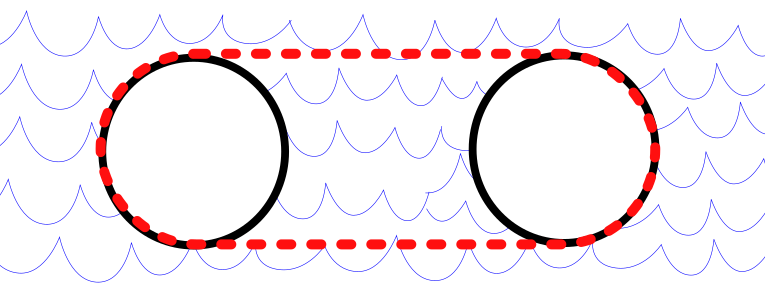
\includegraphics[width=\columnwidth]{figs/stadium-vs-circles}
    \end{column}
  \end{columns}
\end{frame}

\subsection{Four hydrophobic rods}

\begin{frame}[fragile]{}
  \begin{columns}
    \begin{column}{0.5\columnwidth}
      \includegraphics[width=\columnwidth]{figs/density-four-rods}
    \end{column}
    \begin{column}{0.5\columnwidth}
    \includegraphics[width=\columnwidth]{figs/four-rods-energy-vs-distance}
    \end{column}
  \end{columns}
\end{frame}

\subsection{A hydrophobic spherical solute}
\subsection*{}

\begin{frame}[fragile]{Hydrophobic spheres in water}
  \begin{columns}
    \begin{column}{0.5\columnwidth}
      \includegraphics[width=\columnwidth]{figs/density-sphere}
    \end{column}
    \begin{column}{0.5\columnwidth}
      \includegraphics[width=\columnwidth]{figs/sphere-energy-vs-diameter}
    \end{column}
  \end{columns}
\end{frame}


\section{Conclusions}
\subsection*{}

\begin{frame}[fragile]{}
  \begin{block}{}
    \begin{itemize}
    \item Created a classical density functional for water
    \item Expected to be valid over wide range of temperatures and pressures
    \item Models hydrophobic interactions reasonably
    \item Handles both long and short length scales
    \end{itemize}
  \end{block}
  \begin{block}{To do...}
    \begin{itemize}
    \item Realistic dispersive attraction to hydrophobic surfaces
    \item Handle electrostatics
    \item Pseudopotential to couple with electrons in solute
    \end{itemize}
  \end{block}
\end{frame}

\end{document}
